\begin{figure}[ht]
\centering
% Thesis-wide categorical color palette
% Usage: % Thesis-wide categorical color palette
% Usage: % Thesis-wide categorical color palette
% Usage: \input{figures/palette} in any figure file
%
% Muted primary colors -- print-friendly, visually distinct.
% Inspired by Cooper Union's red/blue primaries, softened for
% academic figures. Use palA-palC for data series in scatter
% plots, line charts, bar charts, etc.

\definecolor{palA}{HTML}{1F77B4}   % Tableau blue
\definecolor{palB}{HTML}{D62728}   % Tableau red
\definecolor{palC}{HTML}{2CA02C}   % Tableau green
 in any figure file
%
% Muted primary colors -- print-friendly, visually distinct.
% Inspired by Cooper Union's red/blue primaries, softened for
% academic figures. Use palA-palC for data series in scatter
% plots, line charts, bar charts, etc.

\definecolor{palA}{HTML}{1F77B4}   % Tableau blue
\definecolor{palB}{HTML}{D62728}   % Tableau red
\definecolor{palC}{HTML}{2CA02C}   % Tableau green
 in any figure file
%
% Muted primary colors -- print-friendly, visually distinct.
% Inspired by Cooper Union's red/blue primaries, softened for
% academic figures. Use palA-palC for data series in scatter
% plots, line charts, bar charts, etc.

\definecolor{palA}{HTML}{1F77B4}   % Tableau blue
\definecolor{palB}{HTML}{D62728}   % Tableau red
\definecolor{palC}{HTML}{2CA02C}   % Tableau green

\definecolor{agentblue}{HTML}{4C72B0}
\definecolor{rewardgreen}{HTML}{55A868}
\definecolor{penaltyred}{HTML}{C44E52}

%% Left: grid showing s_21
\begin{subfigure}[b]{0.32\textwidth}
\centering
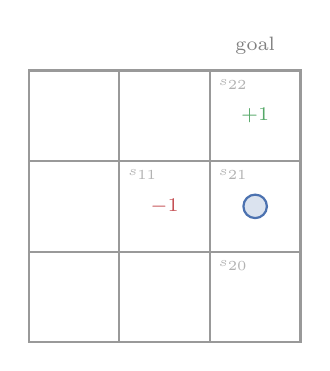
\begin{tikzpicture}[
    cell/.style={minimum size=1.15cm, draw=black!40, thick},
    reward/.style={font=\scriptsize\bfseries},
    agent/.style={circle, draw=agentblue, thick,
                  fill=agentblue!20, inner sep=3pt},
    slbl/.style={font=\tiny, text=black!30, anchor=north west},
]
\def\s{1.15}

% Grid
\foreach \x in {0,1,2} {
    \foreach \y in {0,1,2} {
        \node[cell] (c\x\y) at (\x*\s, \y*\s) {};
    }
}

% Rewards
\node[reward, text=rewardgreen] at (c22) {$+1$};
\node[reward, text=penaltyred] at (c11) {$-1$};

% Labels
\node[slbl] at (c21.north west) {$s_{21}$};
\node[slbl] at (c22.north west) {$s_{22}$};
\node[slbl] at (c11.north west) {$s_{11}$};
\node[slbl] at (c20.north west) {$s_{20}$};

% Agent at s_21
\node[agent] at (c21) {};

% Goal
\node[font=\scriptsize, text=black!50, above=2pt]
    at (c22.north) {goal};

\end{tikzpicture}
\vspace{0.8em}
\subcaption{Agent in $s_{21}$.}
\label{fig:q-grid}
\end{subfigure}
\hfill
%% Right: Q-values from s_21 (star layout)
\begin{subfigure}[b]{0.62\textwidth}
\centering
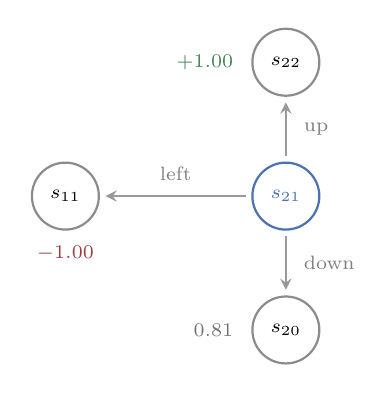
\begin{tikzpicture}[
    state/.style={circle, draw=black!45, thick,
                  minimum size=0.85cm, font=\scriptsize},
    center/.style={state, draw=agentblue,
                   font=\scriptsize\bfseries, text=agentblue},
    arr/.style={->, thick, >=stealth, black!40,
                shorten >=2pt, shorten <=2pt},
    qlbl/.style={font=\scriptsize},
    dirlbl/.style={font=\scriptsize, text=black!50},
]

% Center state
\node[center] (s21) at (0, 0) {$s_{21}$};

% Up -> s_22 (goal, Q = +1.00)
\node[state] (s22) at (0, 1.7) {$s_{22}$};
\draw[arr] (s21) -- (s22);
\node[dirlbl, right=3pt] at (0, 0.85) {up};
\node[qlbl, text=rewardgreen!80!black, left=3pt]
    at (s22.west) {$+1.00$};

% Left -> s_11 (penalty, Q = -1.00)
\node[state] (s11) at (-2.8, 0) {$s_{11}$};
\draw[arr] (s21) -- (s11);
\node[dirlbl, above=2pt] at (-1.4, 0) {left};
\node[qlbl, text=penaltyred!80!black, below=2pt]
    at (s11.south) {$-1.00$};

% Down -> s_20 (Q = 0.81)
\node[state] (s20) at (0, -1.7) {$s_{20}$};
\draw[arr] (s21) -- (s20);
\node[dirlbl, right=3pt] at (0, -0.85) {down};
\node[qlbl, text=black!55, left=3pt]
    at (s20.west) {$0.81$};

\end{tikzpicture}
\vspace{0.8em}
\subcaption{Q-values: same state, different actions.}
\label{fig:q-values-star}
\end{subfigure}

\vspace{0.5em}
\caption{Action values $q_\pi(s_{21}, a)$. From the same state,
  different actions have dramatically different values.}
\label{fig:q-values}
\end{figure}
